\subsection{Task 4.4 -- Continuous Integration}

Workflow \nolinkurl{.github/workflows/ci.yml} tự chạy khi mở hoặc cập nhật pull
request vào \texttt{main}. Hai job \texttt{Build \& Check Backend} và
\texttt{Build \& Check Frontend} dùng Node.js 22, cài phụ thuộc bằng
\texttt{npm ci}, rồi lần lượt chạy lint, unit test và build. Backend tạo
Prisma Client trước khi lint. Job \texttt{API integration and order E2E} dựng
PostgreSQL 16 tạm, áp migration và chạy test tích hợp cùng E2E qua API.

\paragraph{Minh chứng trên PR thanh toán}
\begin{itemize}
  \item \href{https://github.com/PhucTruong11/brewlite-assignment2/pull/1}{PR \#1}
        tích hợp nhánh \texttt{payments} vào \texttt{main}.
  \item \href{https://github.com/PhucTruong11/brewlite-assignment2/actions/runs/42769688179}{CI lượt \#7}
        đạt cả ba job ở commit \texttt{f5dcc2d} với đầy đủ các bước kiểm tra của API và web.
\end{itemize}

Ở lần đối chiếu cấu hình trước đó, \texttt{main} chưa được bảo vệ. Để đáp ứng tiêu chí chặn merge
khi CI thất bại, cần bật branch protection hoặc ruleset trên \texttt{main} và
đặt cả ba job trên làm required checks. Quality gate của workflow phát hành
đã chặn bước triển khai nếu CI thất bại.

\paragraph{Minh chứng CI thành công ngày 19/11/2026}
Lượt CI \#20 của PR \#10 trên nhánh \nolinkurl{feature/reward-voucher-limit}
có trạng thái \texttt{Success}. Cả ba job backend, frontend và integration/E2E
đều đạt; tổng thời gian hiển thị là 1 phút 15 giây.

\begin{reportfigure}
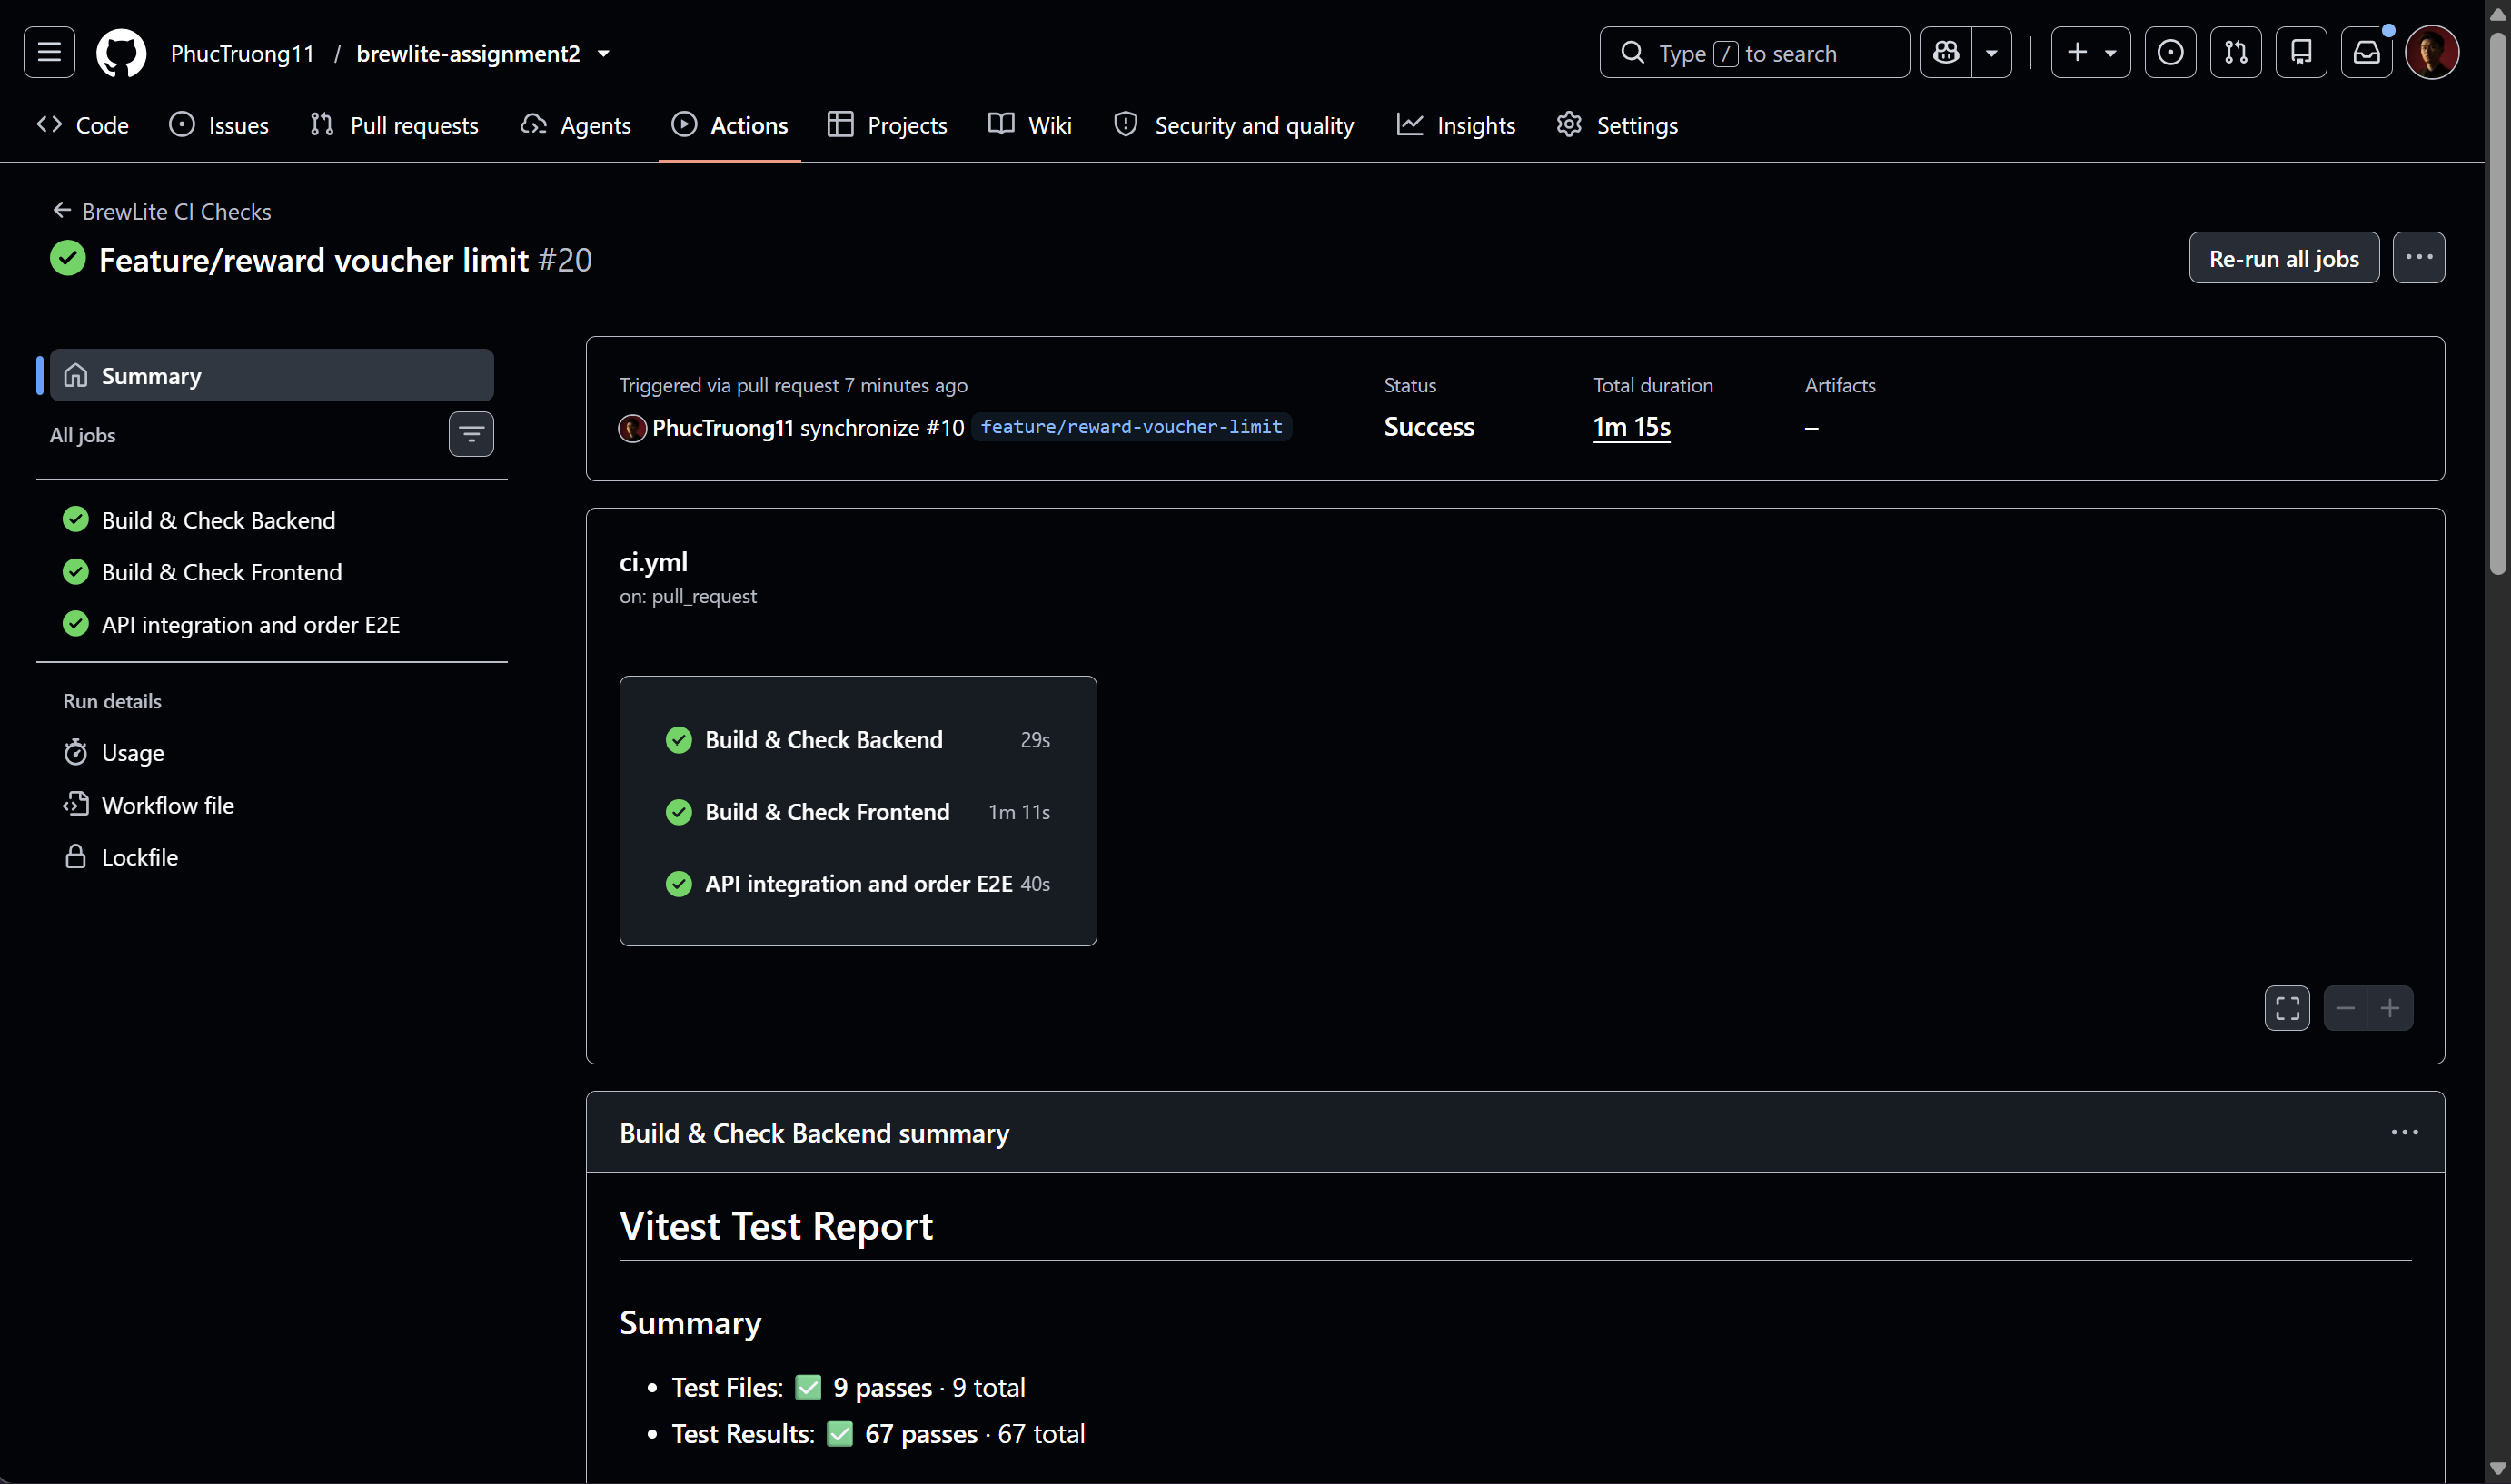
\includegraphics[width=\linewidth,trim=0bp 190bp 0bp 65bp,clip]{../../assets/evidence/ci-success.png}
\par\small\itshape Hình 4.4. Kết quả ba job CI trên pull request
\end{reportfigure}
